\documentclass[12pt, a4paper]{article}
\usepackage{ctex}

\usepackage{geometry}
\geometry{a4paper,left=3.17cm,right=3.17cm,top=2cm,bottom=2cm}
\usepackage{chemformula} %化学公式宏包
\usepackage[version=4]{mhchem} %化学公式宏包
\usepackage{siunitx} %数字，单位宏包
\sisetup{
	separate-uncertainty = true,
	inter-unit-product = \ensuremath{{}\cdot{}}
} %单位间加小圆点
\usepackage{tikz} %Tikz绘图包
\usetikzlibrary{cd}
\usetikzlibrary{chains}
\usetikzlibrary{arrows}
\usetikzlibrary{arrows.meta} %画箭头
\usetikzlibrary{commutative-diagrams} %交换图
\usetikzlibrary{positioning,automata}
\usepackage[all]{xy}
\usepackage{booktabs} %三线表
\usepackage{multirow} %合并单元格
\usepackage{makecell} %表格内强制换行
\usepackage{array}
\usepackage{booktabs} %控制表格行高
\usepackage{colortbl}  %彩色表格需要加载的宏包
\usepackage{pifont} % 圆圈数字
\usepackage{amsmath}
\usepackage{unicode-math}
\usepackage{fontspec} %字体
\usepackage{listings} % 代码
\newcommand*{\cred}{\textcolor{red}}

\setmainfont{Times New Roman}
\setmathfont{XITS Math}
\setCJKmainfont{SimSun}[AutoFakeBold, AutoFakeSlant] 

\setlength{\parindent}{0pt} %无缩进
\usepackage{setspace}
\usepackage{fancyhdr} %设置页码
\usepackage{lastpage} %获取总页数
\pagestyle{fancy} %fancyhdr宏包新增的页面风格
\renewcommand\headrulewidth{0pt} %取消页眉中的装饰分割线
\fancyhf{}
\cfoot{\footnotesize 第 \thepage\ 页(共 \pageref{LastPage}页)}%当前页 of 总页数


%微分符号
\makeatletter
\newcommand*{\dif}{\mathop{}\!\mathrm{d}}
\makeatother

%直立积分
\DeclareSymbolFont{EulerExtension}{U}{euex}{m}{n}
\DeclareMathSymbol{\euintop}{\mathop} {EulerExtension}{"52}
\DeclareMathSymbol{\euointop}{\mathop} {EulerExtension}{"48}
\let\intop\euintop
\let\ointop\euointop

%Python代码排版设置
\lstset{
    language=Python, % 设置语言
 breaklines=true, % 自动换行
 backgroundcolor=\color[rgb]{0.96,0.96,0.96},% 背景颜色
 keywordstyle=\bfseries\color[RGB]{40,40,255}, % 设置关键字为粗体，颜色为 RoyalBlue
 morekeywords={}, % 设置更多的关键字，用逗号分隔
 basicstyle = \linespread{1} \ttfamily, % 设置行距，字体
 emph={left,right,mid}, % 指定强调词，如果有多个，用逗号隔开
    emphstyle=\bfseries\color{Rhodamine}, % 强调词样式设置
    commentstyle=\color{black!50!white}, % 设置注释样式，斜体，浅灰色
    stringstyle=\color{blue!90!black}, % 设置字符串样式
    columns=flexible,
    numbers=left, % 显示行号在左边
    numbersep=2em, % 设置行号的具体位置
    numberstyle=\footnotesize \color{gray}, % 设置行号格式
    xleftmargin=0em, % 左边距
    xrightmargin=0em, % 右边距
    aboveskip=0.5em, % 上边距
    % framexleftmargin=2em, 行号在框内
    framesep=1em, % 设置边框与代码的距离
    frame=shadowbox,rulesep=3pt,rulesepcolor=\color{red!20!green!20!blue!20},% 阴影边框
    showstringspaces = false, % 不显示字符串中的空格
    }

\renewcommand*{\lstlistingname}{Code} % 重定义Listing标题



\begin{document}
\begin{spacing}{1.625}


\centerline{{\Large \bf{河北农业大学}}}

\centerline{\bf{\Large 20\underline{24}年春（\quad ）/秋（\ \surd \ ）学期}}

\centerline{\Large \bf 参考答案及评分标准（A）卷}

\centerline{\bf 开课学院：\underline{\ \ \quad 理工系 \quad \ \ } \quad 出\ \ 题\ \ 人：\underline{\quad \qquad \qquad 张斌\quad \qquad \qquad}}

\centerline{\bf 课\ \ 程\ \ 号：\underline{\ \ H05981011\quad} \quad 课程名称：\underline{\quad \qquad 化学反应工程 \qquad \quad }}

{{\noindent} \hspace{-2em} \rule[0pt]{16cm}{0.15em}}\\

\vspace{-2em}
{\bf 一、简答题（共40分）}

1. (10分) 

\begin{figure}[htpb]
    \centering
    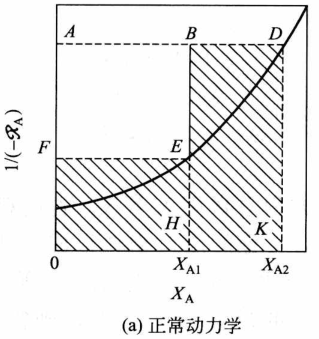
\includegraphics[width=.4\linewidth]{images/串联}
\end{figure}

\qquad 单釜的反应体积与矩形OADK的面积成正比，而两釜串联时总的反应体积与矩形OFEH与HBDK面积之和成正比。显然，面积OADK>（面积OFEH$+$面积HBDK），可见在此情况下两釜串联所需总的反应体积要小于单釜，这一结论可推广到多釜串联，并且串联的釜数越多，所需总的反应体积越小。所以，对于正常动力学，使用多釜串联总是比单釜有利。\hfill $\cdots \cdots \cdots (7\text{分})$

\qquad 但是，釜数多了，相应地管道阀门和控制仪表等也要增多，操作的复杂程度也随之增加，所以，应根据具体情况从经济的角度出发确定最佳的釜数。 \hfill $\cdots \cdots \cdots (3\text{分})$

{\bf 评分标准：}

\qquad 也可回答：单釜操作，始终处于最终转化率下的最小速率下操作；而多釜串联操作，最后一个釜在最小速率下操作，其他釜的速率更高，所以需要的总的反应体积更小。

2. (10分) 

\qquad 绝热温升的意义为：当反应物中的A全部转化时，物系温度升高或降低的度数。\hfill $\cdots \cdots \cdots (4\text{分})$

\qquad 间歇釜式反应器的绝热温升： $\lambda = \frac{n_\mathrm{A0}(-\Delta H_\mathrm{r})}{m_\mathrm{t}\bar{C}_\mathrm{pt}}$  \hfill $\cdots \cdots \cdots (2\text{分})$

\qquad 连续釜式反应器的绝热温升： $\lambda = \frac{c_\mathrm{A0}(-\Delta H_\mathrm{r})}{\rho \bar{C}_\mathrm{pt}}$  \hfill $\cdots \cdots \cdots (2\text{分})$

\qquad 管式反应器的绝热温升： $\lambda = \frac{\omega_\mathrm{A0}(-\Delta H_\mathrm{r})_\mathrm{Tr}}{\bar{C}_\mathrm{pt} M_\mathrm{A}}$  \hfill $\cdots \cdots \cdots (2\text{分})$


3. (10分)

\qquad 目标产物P的选择性：

\qquad $S = \frac{r_\mathrm{P}}{r_\mathrm{P} + r_\mathrm{Q}} = \frac{k_1c_\mathrm{A}c_\mathrm{B}^{0.3}}{k_1c_\mathrm{A}c_\mathrm{B}^{0.3} + k_2c_\mathrm{A}^{0.5}c_\mathrm{B}^{1.3}} = \frac{1}{1 + \frac{k_2}{k_1}c_\mathrm{A}^{-0.5}c_\mathrm{B}}$ \hfill $\cdots \cdots \cdots (4\text{分})$

\qquad $c_\mathrm{A}$越大，P的选择性越大；$c_\mathrm{B}$越大，P的选择性越小。所以A应该在高浓度下操作，B应该在低浓度下操作。 \hfill $\cdots \cdots \cdots (3\text{分})$

\qquad 可行的反应器型式及加料方式有（任选其一）：

\begin{figure}[htpb]
    \centering
    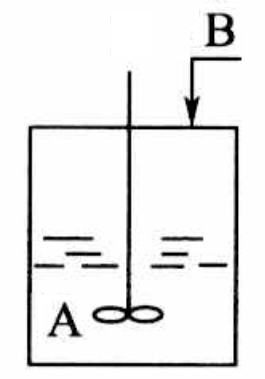
\includegraphics[height=3cm]{images/操作1} \qquad \qquad 
    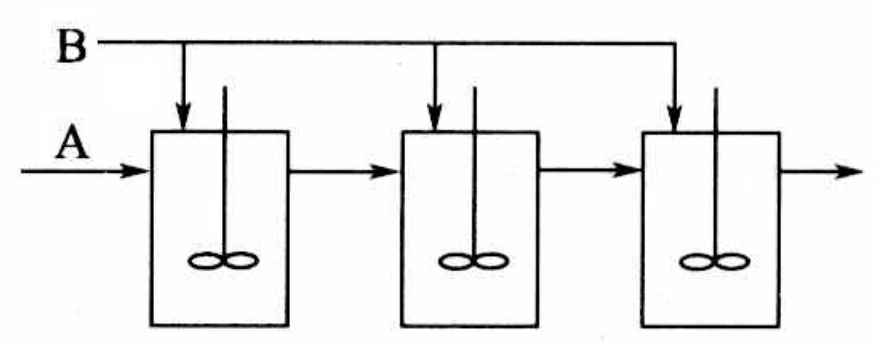
\includegraphics[height=3cm]{images/操作2}
\end{figure}

\hfill $\cdots \cdots \cdots (3\text{分})$

4. (10分)

\qquad 影响连串反应目的产物B的收率的因素有：

\begin{enumerate}
  \item[(1)] $k_2/k_1$的大小，$k_2/k_1$越小，收率越大；\hfill $\cdots \cdots \cdots (4\text{分})$
  \begin{itemize}
    \item 若$E_1>E_2$，温度越高，则$k_2/k_1$越小，收率越大
    \item 若$E_1<E_2$，温度越低，则$k_2/k_1$越小，收率越大
  \end{itemize}
  \item[(2)] 反应器操作方式：在相同的转化率下，间歇釜的收率总是大于连续釜的收率； \hfill $\cdots \cdots \cdots (3\text{分})$
  \item[(3)] 内扩散的影响：内扩散的存在，使目的产物的收率降低，且内扩散的影响越严重，收率降低得越多。\hfill $\cdots \cdots \cdots (3\text{分})$
\end{enumerate}



{\bf 二、计算题（共60分）}

1. (40分) 

(1) $F_\mathrm{A0} = 2400/146/24 = 0.685 \mathrm{\ m^3/h}$  $\hfill \cdots \cdots \cdots (5\text{分})$

$Q_0 = F_\mathrm{A0}/c_\mathrm{A0} = 0.685/0.004/1000 = 0.17 \mathrm{\ m^3/h}$ $\hfill \cdots \cdots \cdots (5\text{分})$

$t = \frac{1}{kc_\mathrm{A0}}\frac{X_\mathrm{A}}{1-X_\mathrm{A}} = \frac{1}{118.2\times 0.004}\times \frac{0.8}{1-0.8} = 8.46 \mathrm{\ h}$ $\hfill \cdots \cdots \cdots (5\text{分})$

$V_\mathrm{r} = Q_0(t+t_0) = 0.17\times (8.46 + 1) = 1.61 \mathrm{\ m^3}$ $\hfill \cdots \cdots \cdots (5\text{分})$

(2) $V_\mathrm{r} = \frac{Q_0 c_\mathrm{A0} X_\mathrm{Af}}{-\mathscr{R}_\mathrm{A}} = \frac{Q_0 c_\mathrm{A0} X_\mathrm{Af}}{kc_\mathrm{A0}^2(1-X_\mathrm{Af})^2} = \frac{0.17\times 0.004 \times 0.8}{118.2\times 0.004^2\times (1-0.8)^2} = 7.19 \mathrm{\ m^3}$ $\hfill \cdots \cdots \cdots (5\text{分})$

(3) $V_\mathrm{r} = Q_0\tau = 0.17\times 8.46 = 1.44 \mathrm{\ m^3}$ $\hfill \cdots \cdots \cdots (5\text{分})$

(4) 活塞流反应器反应体积最小，全混流反应器的反应体积最大，间歇釜的反应体积介于二者之间。$\hfill \cdots \cdots \cdots (5\text{分})$

原因是间歇反应器是变速操作，开始时反应速率最大，终了时最小，而连续釜式反应器是等速操作，且恰恰是在相当于间歇反应器的最小速率下操作，所以连续釜式反应器反应体积大。活塞流反应器是变速操作，开始时反应速率最大，终了时最小，但活塞流反应器没有辅助时间，间歇反应器需要辅助时间，所以活塞流反应器反应体积最小。$\hfill \cdots \cdots \cdots (5\text{分})$

2. (20分) 

(1) $\lambda = 1.013/p = 1.013/(0.1013\times 10^6) = 10^{-5} \mathrm{\ cm}$ $\hfill \cdots \cdots \cdots (1\text{分})$

$\varepsilon_\mathrm{p} = 1 - \frac{\rho_\mathrm{p}}{\rho_\mathrm{t}} = 1 - \frac{1.65}{3.60} = 0.54$ $\hfill \cdots \cdots \cdots (1\text{分})$

$V_\mathrm{g} = \frac{\varepsilon_\mathrm{p}}{\rho_\mathrm{p}} = \frac{0.54}{1.65} = 0.327$ $\hfill \cdots \cdots \cdots (1\text{分})$

$r_\mathrm{a} = \frac{2V_\mathrm{g}}{S_\mathrm{g}} = \frac{2\times 0.327}{200\times 10^4} = 3.27\times 10^{-7} \mathrm{\ cm}$ $\hfill \cdots \cdots \cdots (2\text{分})$

$\frac{\lambda}{2r_\mathrm{a}} = \frac{10^{-5}}{2\times 3.27\times 10^{-7}} = 15.29 > 10$ $\hfill \cdots \cdots \cdots (1\text{分})$

故气体在催化剂内的扩散可按照努森扩散处理。

$D_\mathrm{K} = 9700\times 3.27\times 10^{-7} \sqrt{\frac{773}{58}} = 0.016 \mathrm{cm^2/s}$ $\hfill \cdots \cdots \cdots (1\text{分})$

$D_\mathrm{eA} = \frac{\varepsilon D_\mathrm{K}}{\tau} = \frac{V_\mathrm{g} \rho_\mathrm{p} D_\mathrm{K}}{\tau} = \frac{0.327\times 0.016\rho_\mathrm{p}}{2.5} = 2.09\times 10^{-3}\rho_\mathrm{p}$ $\hfill \cdots \cdots \cdots (1\text{分})$

$k_\mathrm{p} = k_\mathrm{w}\rho_\mathrm{p} = 0.92\rho_\mathrm{p}$ $\hfill \cdots \cdots \cdots (1\text{分})$

$\phi = \frac{d}{6}\sqrt{\frac{k_\mathrm{p}}{D_\mathrm{eA}}} = \frac{0.6}{6}\sqrt{\frac{0.92\rho_\mathrm{p}}{2.09\times 10^{-3}\rho_\mathrm{p}}} = 2.1$ $\hfill \cdots \cdots \cdots (2\text{分})$

$\eta = \frac{1}{\phi}[\frac{1}{\mathrm{tan}h (3\phi)}-\frac{1}{3\phi}] = \frac{1}{2.1}[\frac{1}{\mathrm{tan}h (3\times 2.1)}-\frac{1}{3\times 2.1}] = 0.4$ $\hfill \cdots \cdots \cdots (2\text{分})$

$D_\mathrm{a} = \frac{k_\mathrm{w}}{k_\mathrm{G}a_\mathrm{m}} = \frac{0.92}{0.23} = 4$ $\hfill \cdots \cdots \cdots (1\text{分})$

$\eta_0 = \frac{\eta}{1+\eta D_\mathrm{a}} = \frac{0.4}{1 + 0.4\times 4} = 0.154$ $\hfill \cdots \cdots \cdots (1\text{分})$

(2) 内扩散对多相催化反应的影响程度，可以用内扩散有效因子的数值大小来衡量。有效因子是梯尔模数$\phi$的函数，当催化剂的组成和成型方法，以及反应温度和反应物系的组成均一定时，$\phi$仅取决于催化剂的颗粒粒度，因此，可减小催化剂的粒度来降低内扩散的影响。 $\hfill \cdots \cdots \cdots (5\text{分})$

{\bf 评分标准：}

答案允许存在一定误差。

\end{spacing}
\end{document}